% This work is licensed under the Creative Commons Attribution-NonCommercial 4.0 International License.
% To view a copy of this license, visit http://creativecommons.org/licenses/by-nc/4.0/
% or send a letter to Creative Commons, PO Box 1866, Mountain View, CA 94042, USA.

% !TEX TS-program = xelatex

\documentclass[../Main/chem371-notes.tex]{subfiles}

\setcounter{chapter}{3}
\begin{document}

\chapter{Characterization of stationary points and\\ vibrational analisys}

In this chapter we cover how to characterize stationary points that are found via geometry optimization.
We will discuss harmonic vibrational analysis and the computation of vibrational frequencies.

\section{Characterization of stationary points via the second derivative of the energy}

One of the most important applications of quantum chemistry is to find and identify the stationary points of  potential energy surfaces.
Recall that a stationary point is a molecular geometry for which all first derivatives are null
\begin{equation}
\left.\frac{\partial E(\mathbf{R})}{\partial \mathbf{R}_i}\right|_{\mathbf{R}=\mathbf{R}^*} = 0, i=1,\ldots,N_\mathrm{atoms}
\end{equation}
Points on the PES that correspond minima are stable molecular geometries, while saddle points correspond to transition states.

How can we distinguish minima from transition states? As we discussed in the Chapter on the Born--Oppenheimer approximation, we need to know the curvature of the PES near a stationary point.
It helps that near a stationary point the PES is a \emph{quadratic function} of the nuclear coordinates.
To appreciate this point consider the case of a diatomic molecule A-B with potential energy curve $E(r)$ as a function of the bond distance $r$.
At a stationary point $r^*$, we have that $E'(r) = 0$.
Therefore, if we write the Taylor series for $E(r)$ centered around $r^*$ it can be simplified to 
\begin{equation}
\begin{split}
E(r) & = E(r^*) + \underbrace{E'(r^*)}_{=0} (r - r^*) + \frac{1}{2} E''(r^*) (r - r^*)^2 + \frac{1}{6} E'''(r^*) (r - r^*)^3 + \ldots \\
& = E(r^*) + \frac{1}{2} E''(r^*) (r - r^*)^2 + \ldots
\end{split}
\end{equation}
In the second line we keep only the leading terms in the quantity $r - r^*$ [assuming that $E''(r^*) \neq 0$].
This shows that near the stationary point, the PEC $E(r)$ \emph{looks like a parabola} centered around $r^*$.
The curvature of this parabola depends on $E''(r^*)$, the \emph{second derivative} of the PEC at the stationary point.
If we compute $E''(r^*)$ then we can determine if the stationary point of a diatomic is a minimum or a transition state.

\section{Characterization of stationary points in polyatomic molecules}

For polyatomic molecules the energy is a function of all the atomic coordinates and the Taylor series near a stationary point is given by a more complex formula
\begin{equation}
E(\mathbf{R}) =
E(\mathbf{R})^*
+\frac{1}{2}
\sum_{ij}^{3 N_\mathrm{atoms}} \left.\frac{\partial^2 E(\mathbf{R})}{\partial R_i \partial R_j}\right|_{\mathbf{R}=\mathbf{R}^*} (R_i - R_i^*) (R_j - R_j^*) + \ldots 
\end{equation}
In writing this equation, we use the symbols $R_i$ and $R_j$ to indicate the $x,y,z$ coordinates of all atoms, which in total are $3 N_\mathrm{atoms}$.
This expression is still a quadratic function in the displacements $R_i - R_i^*$ and $R_j - R_j^*$, but the second derivative is replaced with the \emph{Hessian matrix}, the matrix of mixed second derivatives
\begin{equation}
H_{ij} = 
\left.\frac{\partial^2 E(\mathbf{R})}{\partial R_i \partial R_j}\right|_{\mathbf{R}=\mathbf{R}^*}
\end{equation}

To characterize the nature of a stationary point it is necessary to consider the eigenvalues of the Hessian matrix at the stationary point.
If none of the eigenvalues is equal to zero, we can distinguish three cases:
\begin{myitems}
\item If all the eigenvalues are positive, then a stationary point is a local minimum.
\item If some eigenvalues are positive and some are negative, then a stationary point is a saddle point.
Transition states are characterized by only one negative eigenvalue.
\item If the Hessian has only negative eigenvalues then the energy is maximum.
\end{myitems}

\section{Vibrational frequencies}

Once we compute the Hessian matrix, it is possible to compute approximate \emph{harmonic vibrational frequencies}.
Vibrations in a molecule are due to the motion of the nuclei.
So to obtain information about vibrations we have to solve the nuclear Schr\"{o}dinger equation assuming the Born--Oppenheimer approximation
\begin{equation}
[\hat{T}_\mathrm{n} + E(\mathbf{R}) ] \Psi_v(\mathbf{R}) = E_v \Psi_v(\mathbf{R})
\end{equation}
This equation describes the quantum mechanical states of nuclei that move on the potential energy surface $E(\mathbf{R})$.
The electrons never appear explicitly in this equation, but their effect is implicitly included in the PES (which we get from the electronic Schr\"{o}dinger equation).

Solving  the nuclear Schr\"{o}dinger equation near a stationary point is particularly simple because the potential is quadratic
\begin{equation}
E(\mathbf{R}) =
E(\mathbf{R})^*
+\frac{1}{2}
\sum_{ij} H_{ij} (R_i - R_i^*) (R_j - R_j^*) 
\end{equation}

For a diatomic molecule, the Hamiltonian is equivalent to that of a \emph{quantum harmonic oscillator}.
This can be more easily seen if we change coordinate from $r$ to $x = r - r^*$ 
\begin{equation}
\begin{split}
\hat{T}_\mathrm{n} + E(\mathbf{R}) & = -\frac{1}{2 \mu} \frac{d^2}{dr^2} + 
 \underbrace{E(r^*)}_{V_0} + \frac{1}{2} E''(r^*) (r - r^*)^2 \\
 & = \underbrace{\left( -\frac{1}{2 \mu} \frac{d^2}{dx^2} 
+ \frac{1}{2} k x^2 \right)}_{\text{harmonic oscillator}} + V_0
\end{split}
\end{equation}
where $V_0$ is the energy at the bottom of the well (the energy you get when you optimize the geometry of the diatomic molecule), $\mu = (M_A + M_B) / M_A M_B$ is the reduced mass of the diatomic molecule, and $k = E''(r^*)$ is the force constant.

\mfigure{
\centering{
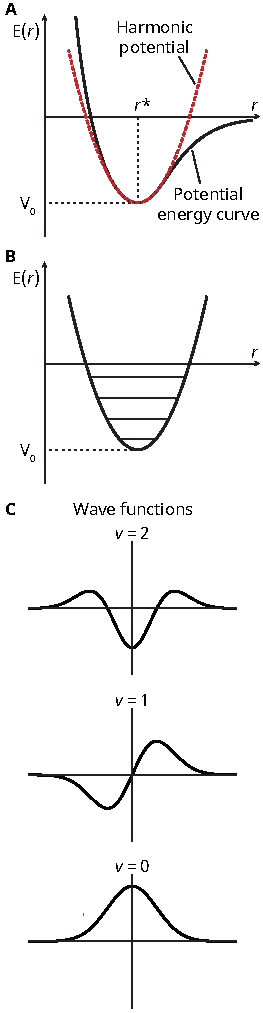
\includegraphics[width=1.75in]{img/diatomic.pdf}
}
\captionof{figure}{The potential energy surface of a diatomic molecule near the equilibrium bond distance ($r_\mathrm{eq}$) can be approximated by a quadratic function (parabola, see \textbf{A}). \textbf{B} and \textbf{C} show the energy levels and wave functions of the diatomic molecule vibrating with a quadratic potential.}
\label{fig:4:diatomic}
}

The quantum harmonic oscillator is one of those few problems for which we know analytical solutions to the Schr\"{o}dinger equation.
The eigenvalues of the quantum harmonic oscillator are given by (in atomic units)
\begin{equation}
E_v = V_0 + \sqrt{\frac{k}{\mu}} \left(v + \frac{1}{2}\right)
= V_0 +  \omega \left(v + \frac{1}{2}\right), \quad v = 0,1,2,\ldots
\end{equation}
where $\omega$ is the angular frequency of the oscillator and $v$ is the vibrational quantum number.
The ground state of the harmonic oscillator (the minimum energy) is obtained for $v = 0$ and it is equal to
\begin{equation}
E_0 = V_0 +  \frac{1}{2}\omega
\end{equation}
Note that this quantity is always \emph{higher} than the energy at the bottom of the potential ($V_0$) by an amount equal to $\frac{1}{2}\omega$!
This amount of energy is called the \emph{zero-point energy}, and it is due to the quantum nature of vibrations.

For polynuclear molecules, the solution to the nuclear Schr\"{o}dinger equation can be found by diagonalization of the mass-weighted Hessian matrix
\begin{equation}
\tilde{H}_{ij} = \frac{H_{ij}}{\sqrt{M_i M_j}}
\end{equation}
Diagonalizing the mass-weighted Hessian matrix means finding a set of eigenvectors $\mathbf{u}^{(\alpha)}$ and corresponding eigenvalues $\lambda_\alpha$ that satisfy the equation
%\mnote{In matrix notation this equation corresponds to
%$\tilde{\mathbf{H}} \mathbf{u}^{(\alpha)} = \lambda_\alpha \mathbf{u}^{(\alpha)}$}
\begin{equation}
\sum_{j} \tilde{H}_{ij} u^{(\alpha)}_{j} = \lambda_\alpha u^{(\alpha)}_{i}
\end{equation}
Each eigenvector/eigenvalue pair corresponds to a molecular vibrational mode $\alpha$, which we call a \emph{normal vibrational mode}.
Each mode behaves as an independent harmonic oscillator with angular frequency
\begin{equation}
\omega_\alpha = \sqrt{\lambda_\alpha}
\end{equation}
and has an associated quantum number $v_\alpha = 0, 1, 2, \ldots$.

Once the mass-weighted Hessian matrix is diagonalized, the eigenvalues of the nuclear Sch\"{o}dinger equation (nuclear energy levels) are given by
\begin{equation}
E_v = V_0 + \sum_{v_\alpha} \omega_\alpha \left(\frac{1}{2} + v_\alpha\right)
\end{equation}
where the quantities $v_\alpha$ are the quantum numbers for each vibrational mode.
For a general molecule, the zero-point energy is given by
\begin{equation}
E_0 = V_0 + \frac{1}{2}  \sum_{v_\alpha} \omega_\alpha
\end{equation}
which again we see is higher than the energy at the bottom of the well.

The harmonic vibrational analysis introduced here can be performed with the majority of quantum chemistry codes.
There are three main applications of a vibrational analysis
\begin{myitems}
\item The \emph{sign} of the eigenvalues $\lambda_\alpha$ tell us information about the curvature of the PES at the stationary point.
If all the $\lambda_\alpha$ are positive the stationary point is a minimum. \emph{This corresponds to the case where all the frequencies are real}, since $\omega_\alpha = \sqrt{\lambda_\alpha}$.
The presence of one or more \emph{negative} eigenvalues indicates that there is a vibrational mode with a negative curvature.
In this case a stationary point is a transition state.
This case corresponds to finding an imaginary frequency since if an eigenvalue $\lambda_\alpha$ is negative, its square root will be an imaginary number, $\omega_\alpha = i \sqrt{|\lambda_\alpha|}$.

\item The \emph{value} of the individual vibrational frequencies $\omega_\alpha$ \emph{approximate the vibrational frequencies measured in IR absorption spectroscopy}.
The eigenvectors of the mass-weighted Hessian tell us how the atoms are displaced in a vibrational mode, and can therefore tell us if a given mode is a bond stretching mode, a bending mode, etc.

\item The \emph{sum} of the vibrational frequencies tell us information about the zero-point energy of a molecule.
Accurate thermodynamic computations \emph{must} include the zero-point energy to include nuclear vibrational effects and ultimately achieve good agreement with experiment. We will come back to this topic later.
\end{myitems}

\begin{ibox}
An important thing to remember is that a harmonic vibrational analysis is meaningful only if:
\begin{enumerate}
\item The geometry used to compute the frequencies is \emph{optimized}
\item The computation of the Hessian is \emph{performed at the same level of theory}
\end{enumerate}
For example, if you compute the geometry with the B3LYP density functional using the def2-TZVP basis, then a subsequent frequency computation \emph{mustbe done at the same level of theory starting from the optimized geometry}.
\end{ibox}

\section{Example: vibrational analysis of water}

\mfigure{
\centering{
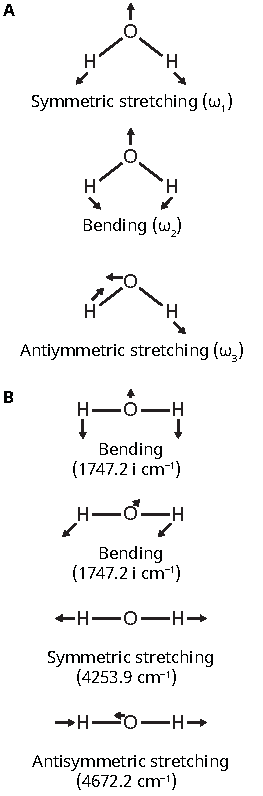
\includegraphics[width=1.75in]{img/h2o.pdf}
}
\captionof{figure}{Normal modes of water at the equilibrium geometry (\textbf{A}) and at the linear transition state (\textbf{B}) computed with Hartree--Fock theory and the def2-TZVP basis.}
\label{fig:4:h2o}
}

The example below shows the vibrational analysis of the water molecule using Hartree--Fock and the def2-TZVP basis.
The vibrational analysis shows that six modes are classified as ``low-frequency'' because they are close to zero (post-proj low-frequency mode).
Some of these numbers are imaginary, and that's due to small numerical noise.
These six low-frequency modes are trivial modes corresponding to three translations (along the $x$, $y$, or $z$ direction) and three rotations (around the $x$, $y$, or $z$ axis), hence the label ``TR''.

Modes 7, 8, and 9 corresponds to three molecular vibrational modes.
Starting from the highest frequency mode, we have
\begin{myitems}
\item  Mode 9 ($\omega_3$ = 4213.5 cm$^{-1}$), an antisymmetric stretching of the two \ce{O-H} bonds.
\item Mode 8 ($\omega_1$ = 4111.5 cm$^{-1}$), a symmetric stretching of the two \ce{O-H} bonds.
\item Mode 7 ($\omega_2$ = 1734.7 cm$^{-1}$), a \ce{H-O-H} bending mode. 
\end{myitems}
Each normal mode has also an associated symmetry. The A$_1$ modes correspond to \emph{totally symmetric modes}.
This means that if we transform the modes according to any of the symmetries of water, the normal mode does not change.
Mode 9 is of type B$_2$, which means that if we rotate the molecule by 180\textdegree{} along the vertical axis that includes the oxygen atom, then the normal mode changes sign.

The calculation also tells us the IR activity (measured in km/mol) of each normal mode. This information allows us to predict or relate our results to an experimental spectrum. All three normal modes are active, with mode 7 and 9 being the most intense.

\begin{small}
\begin{verbatim}
  ==> Harmonic Vibrational Analysis <==
...
  post-proj low-frequency mode:    0.0001i [cm^-1] (TR)
  post-proj low-frequency mode:    0.0001i [cm^-1] (TR)
  post-proj low-frequency mode:    0.0000i [cm^-1] (TR)
  post-proj low-frequency mode:    0.0000i [cm^-1] (TR)
  post-proj low-frequency mode:    0.0000i [cm^-1] (TR)
  post-proj low-frequency mode:    0.0001  [cm^-1] (TR)

  Vibration                       7                   8
  Freq [cm^-1]                1734.7180           4111.5086
  Irrep                           A1                  A1
  Reduced mass [u]              1.0835              1.0444
  Force const [mDyne/A]         1.9210             10.4022
  Turning point v=0 [a0]        0.2531              0.1674
  RMS dev v=0 [a0 u^1/2]        0.1863              0.1210
  IR activ [km/mol]            101.9411            17.0610
  Char temp [K]               2495.8730           5915.5454
  -------------------------------------------------------------
      1   O               -0.00 -0.00 -0.07    0.00  0.00  0.05
      2   H                0.00  0.42  0.56    0.00  0.59 -0.39
      3   H               -0.00 -0.42  0.56   -0.00 -0.59 -0.39
      
      
        Vibration                 9           
  Freq [cm^-1]                4213.5468       
  Irrep                           B2          
  Reduced mass [u]              1.0839        
  Force const [mDyne/A]        11.3375        
  Turning point v=0 [a0]        0.1624        
  RMS dev v=0 [a0 u^1/2]        0.1195        
  IR activ [km/mol]             76.6343        
  Char temp [K]               6062.3558       
  -----------------------------------------
      1   O               -0.00 -0.07  0.00   
      2   H               -0.00  0.57 -0.42   
      3   H                0.00  0.57  0.42   
\end{verbatim}
\end{small}

The information listed at the bottom shows how each atom moves in each of the normal modes.
For each atom, each triplet of numbers under a normal mode indicate how much is the atom displaced in the $x$, $y$, and $z$ directions.
This information can be used to analyze the nature of the normal modes in a molecule.

If we now repeat the same computation for linear water (after optimizing the geometry) we find seven low-frequency modes, two of which have a large imaginary frequency, $\omega$ = 1747.2 i cm$^{-1}$.
The presence of these two imaginary modes tells us that linear water is a transition state.
The two imaginary frequencies are two orthogonal bending modes that connect linear \ce{H-O-H} to the bent ground state.
If we were to follow these modes and optimize the geometry, we would obtain back the bent structure.

\begin{small}
\begin{verbatim}
  ==> Harmonic Vibrational Analysis <==

...
  post-proj low-frequency mode: 1747.1869i [cm^-1] (V)
  post-proj low-frequency mode: 1747.1869i [cm^-1] (V)
  post-proj low-frequency mode:    0.0000i [cm^-1] (TR)
  post-proj low-frequency mode:    0.0000  [cm^-1] (TR)
  post-proj low-frequency mode:    0.0000  [cm^-1] (TR)
  post-proj low-frequency mode:    0.0000  [cm^-1] (TR)
  post-proj low-frequency mode:    0.0000  [cm^-1] (TR)

  Vibration                       1                   2           
  Freq [cm^-1]                1747.1869i          1747.1869i                 
  Irrep                                                                             
  Reduced mass [u]              1.1259              1.1259                      
  Force const [mDyne/A]        -2.0250             -2.0250                     
  Turning point v=0 [a0]        0.0000              0.0000                      
  RMS dev v=0 [a0 u^1/2]        0.0000              0.0000                      
  IR activ [km/mol]            551.4304            551.4304                     
  Char temp [K]                 0.0000              0.0000                  
  
  Vibration                       8                   9           
  Freq [cm^-1]                4253.9467           4672.2019       
  Irrep                          Ag                 B1u          
  Reduced mass [u]              1.0078              1.1259        
  Force const [mDyne/A]        10.7453             14.4807        
  Turning point v=0 [a0]        0.1676              0.1513        
  RMS dev v=0 [a0 u^1/2]        0.1190              0.1135        
  IR activ [km/mol]             0.0000            829.5184       
  Char temp [K]               6120.4822          6722.2582       
\end{verbatim}
\end{small}

\begin{summary}
\item The potential energy surface near stationary points can be approximated by a quadratic function of the energy.
\item The Hessian of the energy (the matrix of second partial derivatives) provides information about the curvature of the PES. Its eigenvalues allow us to distinguish between (local) minima (all eigenvalues positive) and transition states (one or more negative eigenvalues).
\item The solutions of the nuclear Schr\"{o}dinger equation near a stationary point (assuming a quadratic approximation to the energy) are called \emph{normal modes}.
\item Normal modes tell information about the nature of stationary points, IR spectroscopy, and the zero-point energy.
\end{summary}


\end{document}